%===========================================================
%                              Choix de track
%===========================================================
% Une des trois options 'parallelisme', 'architecture', 'systeme' 
% doit être utilisée avec le style compas2017
\documentclass[parallelisme]{compas2017}

\usepackage[utf8]{inputenc}
\usepackage[T1]{fontenc}

\usepackage{url}
\usepackage{graphicx}
\usepackage{caption}
\usepackage{subcaption}
\usepackage{subfig}
\usepackage{wrapfig}
\usepackage{multirow}
\usepackage{boxedminipage}
\usepackage{xspace}
\usepackage{listings}
\usepackage{listingsutf8}
\usepackage{verbatim}
\usepackage{parcolumns}
\usepackage{color}
\usepackage[usenames,dvipsnames,svgnames,table]{xcolor}
%Prevents floating item to "jump" between sections
\usepackage[section]{placeins}
\usepackage{booktabs}
\usepackage{tkz-graph}
\usepackage{setspace}
%\setstretch{0.95}




\renewcommand{\ttdefault}{pcr}
\lstset{
	tabsize=4,
%	frame=single,
	breaklines=true,
	basicstyle=\ttfamily,
	frame=tb,
	framerule=0.2pt,
%	frameround={tttt},
	showstringspaces=false,
	language=c,
%	linewidth=0.95\textwidth,
	keywordstyle=\color{black}\bfseries,
%	keywordstyle=\color{blue},
	commentstyle=\color{OliveGreen},
	stringstyle=\color{red}\itshape,
	inputencoding=utf8/latin1,
	numbers=left,
	numberstyle=\tiny,
	numbersep=5pt,
% OMP define
emph={\#,pragma, taskwait, omp, task, depend}, emphstyle=\color{RoyalBlue}\bfseries,
emph={omp_affinitykind_t,uintptr_t}, emphstyle=\color{Black}\bfseries,
emph={[2]in,inout,out,cw,data,node,thread}, emphstyle={[2]\color{BrickRed}\bfseries},
emph={[3]tied,untied,shared, firstprivate, private}, emphstyle={[3]\color{Gray}\bfseries},
emph={[4]lu0,fwd,bdiv,bmod}, emphstyle={[4]\color{DarkGreen}\bfseries},
emph={[5]affinity, omp_get_numa_num, omp_get_num_numas, omp_get_numa_from_data,omp_set_task_affinity}, emphstyle={[5]\color{DarkViolet}\bfseries},
    %moredelim=**[is][\only<3>{\color{red}}]{@}{@},
}
\lstdefinestyle{smaller}{basicstyle=\scriptsize\ttfamily}
\lstMakeShortInline|


\newcommand{\kaapi}{\textsc{\mbox{XKaapi}}\xspace}

\newcommand{\libXKOMP}{\textsc{libKOMP}\xspace}


%===========================================================
%                               Title
%===========================================================

\toappear{1} % Conserver cette ligne pour la version finale

\begin{document}

\title{Étude de l'impact d'une clause d'affinité sur les performances et l'énergie
dans un support exécutif OpenMP}

\author{Philippe Virouleau}
\address{Inria,\\
   Univ. Grenoble Alpes,  CNRS, Grenoble Institute of Technology, LIG, Grenoble, France\\
   philippe.virouleau@inria.fr\\
}
\date{\today}



\maketitle
%\vspace*{-2ex}

%===========================================================         %
%R\'esum\'e
%===========================================================  
\begin{abstract}
La norme OpenMP 4.0 a introduit les tâches avec dépendances, qui permettent au
programmeur d'exprimer du parallélisme à grain fin.

Contrôler la localité des données lors de l'exécution de ces tâches
est l'un des facteurs clés pour obtenir un bon niveau de performances sur des architectures NUMA.
Dans ce domaine, OpenMP ne propose pas encore beaucoup de flexibilité au programmeur,
ce qui laisse au support exécutif la responsabilité de décider où les tâches doivent
être exécutées.

Cet article présente la description, l'implémentation, et l'évaluation d'une
nouvelle clause \emph{affinity} pour les tâches, qui
est actuellement en discussion au sein du comité du langage OpenMP.
Cette clause permet au programmeur de donner des informations au support exécutif
à propos du placement de la tâche au cours de l'exécution, ce qui peut également
être utilisé par le programmeur pour contrôler le placement de données sur
l'architecture.
Il présente également des classes d'applications qui pourraient bénéficier d'une
telle flexibilité de placement de tâches et de données, ainsi qu'un aperçu rapide
de l'impact sur la consommation énergétique.

  \MotsCles{OpenMP, affinité, support exécutif, NUMA, énergie}
\end{abstract}


%=========================================================
%\vspace*{-2ex}
\section{Introduction}
%\vspace*{-1ex}
%=========================================================

Les architectures à temps d'accès mémoire non uniforme (NUMA) sont
aujourd'hui le choix le plus populaire pour créer des grosses machines à mémoire
partagée. Le temps d'accès à la mémoire dépend de la distribution physique des
données, leur placement et leur localité durant la vie du programme sont
donc des points clés pour améliorer la scalabilité et les performances.

Les environnements de programmation parallèle tels que OpenMP, OpenCL, ou TBB sont devenus très
populaires pour exploiter les machines à mémoire partagée avec plusieurs centaines de cœurs.
La plupart d'entre eux fournissent également
un moyen d'équilibrer dynamiquement la charge de travail sur tous les processeurs,
mais aucun d'entre eux ne fournit de moyen assez flexible de gérer la localité
des données sur des systèmes NUMA.

Le concept de \emph{places} ajouté avec OpenMP 4.0 permet d'associer les threads
d'une région parallèle à un ensemble
de cœurs physiques, ce qui permet d'aider à conserver l'affinité d'un thread avec la mémoire.
Néanmoins cela n'est pas suffisant pour améliorer les performances des applications
à base de tâches, au cours desquelles les tâches sont ordonnancées dynamiquement sur les différent threads.

Cet article présente un contrôle du placement des tâches et des données
dans un support exécutif OpenMP, en implémentant une clause \emph{affinity}.
Il montre également comment cette information peut être utilisée à l'exécution pour
améliorer la localité des données, ce qui a un impact direct sur les performances
et la consommation énergétique.
L'évaluation de ces travaux a été effectuée sur deux machines NUMA : une disposant de 192
cœurs, et l'autre disposant de 48 cœurs.

Le plan de cet article est le suivant :
la partie~\ref{sec:background},
contient quelques informations essentielles sur les architectures NUMA et
les outils utilisés.
La partie~\ref{sec:contributions} regroupe la description de la syntaxe
et de l'implémentation d'une clause \emph{affinity}.
La partie~\ref{sec:experiment}
présente les évaluations de performances sur des applications de types Stencil
et d'algèbre linéaire.
Enfin les travaux de l'état
de l'art sont présentés dans la partie~\ref{sec:related-work}, avant les travaux
en cours et la conclusion.


%\vspace*{-2ex}
\section{Cible et outil}
%\vspace*{-1ex}
\label{sec:background}

\subsection{Description des systèmes NUMA et de leur exploitation}


Les architectures NUMA sont des machines à mémoire partagée dont les cœurs
physiques ainsi que la mémoire sont divisés en plusieurs ensembles ("nœuds"),
interconnectés entre eux de manière transparente pour l'utilisateur.

Afin d'exploiter de telles architectures, le programmeur a besoin
d'une part d'exprimer beaucoup de parallélisme à grain fin, pour profiter au
maximum du nombre important de processeurs disponibles; et d'autre part de contrôler
l'exécution de l'application, en particulier la manière dont sont distribuées
et accédées les données.

Les environnements de programmation parallèle à base de tâches fournissent un moyen
d'exprimer le parallélisme à grain fin. OpenMP~\cite{openmp40}, le standard utilisé
en pratique pour la programmation des architectures à mémoire partagée, supporte
le parallélisme à base de tâches avec dépendances de données depuis la version 4.0.

\subsection{Mesure et consommation énergétique}

Les mesures énergétiques effectuées ont été basées sur la fonctionnalité Intel RAPL
(Running Average Power Limit), disponible sur les processeurs Intel de nos machines.
Cette fonctionnalité expose la consommation de certains composants sur le socket
(comme l'ensemble du processeur - \emph{package} - et la DRAM) à travers les 
MSR (Model Specific Registers).

La précision de ces compteurs dépend du modèle de processeur, les différences
entre Sandy Bridge et Haswell on été étudié dans~\cite{7284406,6148200}.

Un petit outil a été conçu pour accéder périodiquement aux informations des registres MSR :
basé sur l'API de LIKWID~\cite{DBLP:journals/corr/abs-1104-4874}, il récupère les
informations pour la totalité du processeur (|PWR_PKG_ENERGY|), pour les coeurs
(\verb/PWR_PP0_ENERGY/), et pour la DRAM (\verb/PWR_DRAM_ENERGY/).
Cet outil récupère les valeurs toute les 100ms, et les associe à un timestamp.


%\vspace*{-2ex}
\section{Extension d'OpenMP pour supporter l'affinité}
%\vspace*{-2ex}
\label{sec:contributions}

Cette partie détaille l'introduction du mot clé |affinity|, ainsi que l'implémentation côté support
exécutif pour exploiter cette fonctionnalité.

%\vspace*{-1ex}
\subsection{Description d'une clause affinité}

Les deux principaux composants des architectures NUMA que l'on considère pour
cette proposition sont les cœurs et les nœuds. Un point clé pour obtenir
de bonnes performances sur des architectures NUMA est de garantir qu'une tâche
s'exécute \emph{proche} de ses données.
On distingue donc trois types d'affinité que le programmeur pourrait avoir besoin
d'exprimer :

\begin{description}
    \item [affinité à un thread :]
      le support exécutif devrait essayer d'ordonnancer la tâche sur le thread donné.
       
    \item [affinité à un nœud NUMA :]
      le support exécutif devrait essayer d'ordonnancer la tâche sur n'importe
      quel thread du nœud NUMA donné.

    \item [affinité à une donnée :]
      quand une tâche devient prête pour l'exécution, le support exécutif devrait
      l'ordonnancer sur n'importe quel thread attaché au nœud NUMA sur lequel
      la donnée a été physiquement allouée.
\end{description}

De plus, le programmeur peut indiquer si cette affinité est \emph{stricte},
indiquant que la tâche \textbf{doit} s'exécuter sur la ressource indiquée.
Si le programmeur n'indique pas une affinité stricte, l'ordonnanceur peut décider
d'exécuter la tâche sur une ressource différente, pour assurer l'équilibrage de
charge par exemple.

Cette extension visant les constructions de type tâche, elle a été implémentée
comme une nouvelle clause pour la directive |task|. La syntaxe proposée est la
suivante :

\begin{lstlisting}
affinity([node | thread | data]: expr[, strict])
\end{lstlisting}

Si \emph{expr} désigne un id de thread, elle devrait désigner l'id de thread dans
les |OMP_PLACES| définies pour la \textit{team} courante. Exemple : si les places
sont |"{2},{5},{8}"|, et que \emph{expr} est évaluée comme valant 0, l'id du thread désigné est |"{2}"|.

Si \emph{expr} désigne un id de nœud NUMA, elle devrait désigner un id de nœud
dans l'ensemble des nœuds NUMA construit à partir de la liste des |OMP_PLACES|.

Si \emph{expr} désigne une donnée, elle devrait être une adresse mémoire.
Si le nœud NUMA associé à la donnée ne peut être déterminé, le nœud par défaut
est le premier dans la \textit{team} OpenMP.

Si \emph{expr} désigne une ressource hors limites, la valeur est prise modulo le
nombre de ressources.

\subsection{Implémentation dans un compilateur et un support exécutif}
\label{subsec:implem-runtime}

La clause a été implémentée dans le frontend de Clang, et le support
exécutif distribué avec LLVM (basé sur le support exécutif d'Intel) a été modifié
pour supporter l'affinité.
Ce support exécutif ayant une vision uniforme de la machine, il a fallu premièrement l'étendre
pour mettre en place une vision hiérarchique de la machine.
Cela a été fait en intégrant la gestion des queues hiérarchiques présente dans
\libXKOMP~\cite{Durand2013,libkomp}, ainsi que la gestion du vol de travail présent
dans \kaapi~\cite{Bleuse2014,parco2015}.

Ensuite le support exécutif ne proposait qu'une stratégie de vol de travail aléatoire,
il fallait donc ajouter des stratégies de vol pour prendre en compte les différentes
queues hiérarchiques.
Cela a été fait en intégrant des précédents travaux concernant des stratégies
d'ordonnancement~\cite{Virouleau:2016:UDD:2990973.2990982} sur architectures
NUMA.
L'implémentation de la clause \verb/affinity/ vient se greffer par dessus ces travaux,
en ajoutant des stratégies de vol de travail.

%\vspace*{-2ex}
\section{Résultat expérimentaux}
%\vspace*{-2ex}
\label{sec:experiment}

Les expériences ont été effectuées sur deux machines :

Une SGI UV2000, constituée de
24 nœuds NUMA, possédant chacun un processeur Intel Xeon E5-4640 à 8 cœurs,
le tout formant un total de 192 cœurs. Cette machine dispose de 31Go de RAM
par nœud, pour un total de 744Go. Le nom Intel192 sera utilisé pour faire
référence à cette machine dans l'article.

Une SuperMicro 4048B-TR4FT, constituée de 4 nœuds NUMA, possédant chacun un
processeur Intel Haswel-EX E7-4830 à 12 cœurs, le tout formant un total de 48 cœurs.
Chacun des nœuds dispose de 64Go de RAM, pour un total de 256Go.
Sur cette machine l'hyperthreading peut être activé pour atteindre un nombre de 96 cœurs.
Le nom Intel48 sera utilisé pour faire référence à cette machine dans l'article.

Deux types d'applications ont été considérés pour montrer l'intérêt d'une clause affinité :
\begin{itemize}
    \item Les applications de type Stencil, illustrées ici par le programme Jacobi.
    \item Les applications d'algèbre linéaires, illustrées ici par les factorisations de Cholesky et QR.
\end{itemize}


Ces applications sont tirées de la suite de benchmarks KASTORS~\cite{virouleau:hal-01081974}.  
Elles ont été évaluées sur trois supports exécutifs différents : libGOMP, le support
exécutif de Gcc (6.3) ; libOMP, le support exécutif de Clang (4.0), et libKOMP, décrit
dans la section~\ref{subsec:implem-runtime}.
Les résultats présentés sont des moyennes sur 6 runs, les barres d'erreurs sont
affichées sur les courbes et permettent de montrer la stabilité des résultats.

\subsection{Stencil}

Le noyau Jacobi est une application de type stencil 2D.
Les performances de ce type d'application sont très dépendantes de la réutilisation
du cache entre les itérations ; les implémentations à base de boucles OpenMP sont
donc généralement beaucoup plus efficaces que celles à base de tâches, vu que
pour ces dernières l'ordonnanceur peut déplacer deux tâches qui devraient rester
sur le même cœur.

Plusieurs implémentations de ce noyau ont été comparées. Une version itérative
utilisant des constructions de type \textit{for} pendant l'initialisation et le
calcul (nommée "For"). Une version à base de tâches avec dépendances pour l'initialisation
et le calcul (nommée "Dep. Tasks"). Une version à base de tâches avec dépendances
incluant des affinités (nommée "Dep. Tasks + Affinity").

Cette dernière version utilise des affinités strictes pour l'initialisation et le calcul,
indiquant précisément la ressource sur laquelle la tâche devrait s'exécuter en
fonction du nombre de threads.
Parmi les expériences effectuées, les résultats présentés en figure~\ref{fig:eval-jacobi}
donnent un bon aperçu des comportements observés sur les différents support exécutifs.


\begin{figure}[t]
%\vspace*{-4ex}
  \centering
  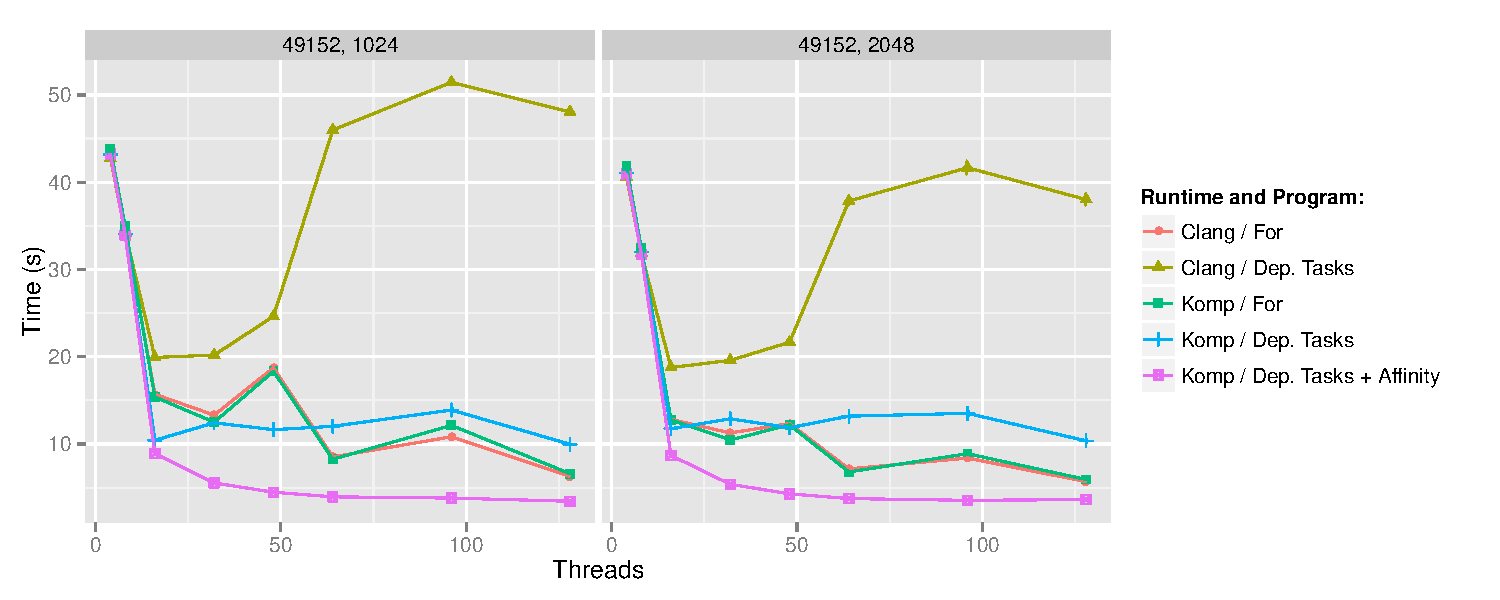
\includegraphics[scale=0.55]{./graphs/jacobi_scale_iomp_komp.pdf}
%\vspace*{-2ex}
  \caption{Performance de Jacobi sur Intel192 avec une taille de matrice de 49152}
%\vspace*{-6ex}
\label{fig:eval-jacobi}
\end{figure}

Le premier commentaire que l'on peut faire est que l'application ne passe
globalement pas très bien à l'échelle, peu importe le support exécutif utilisé.
Le programme est \textit{memory bound} et on ne peut pas faire beaucoup plus
que s'assurer que le calcul s'effectue proche des données.

La version tâche avec dépendances de base n'est pas très performante (c'est même
catastrophique avec le support exécutif de Clang !). Ici la seule explication
derrière ces performances est le fait que la stratégie de sélection de victimes dans le vol de travail est complètement aléatoire
dans libOMP, alors qu'il y a une sélection hiérarchique dans libKOMP. Cela n'empêche pas
que pour les deux supports exécutif, certains vol de tâches dégradent les performances !

On remarque que la version avec affinité offre les meilleures performances grâce à un contrôle
strict de l'association entre une tâche et ses données.

Étonnamment la version itérative "For" ne présente pas les même résultats que la version
avec affinité : un meilleur découpage des itérations devrait être à même de palier
à ce problème. Note : les pics à 48 et 96 threads sont probablement dû au fait que
ces nombres ne sont pas des puissances de 2, ce qui ne permet pas automatiquement un découpage
des itérations optimal correspondant à la topologie.


\subsection{Algèbre linéaire}

L'objectif de cette section est double : observer l'impact de l'affinité sur les
performances, et faire une première observation de l'impact potentiel sur
l'énergie consommée.

La version "affinité" des factorisations de Cholesky et QR implémente une affinité
assez similaire à l'\textit{owner compute rule} présente dans HPF~\cite{HPF} :
les différents noyaux de chaque application sont annotés d'une affinité sur
les données en écriture pour ce noyau.
L'initialisation des blocs de données a été fixée via une affinité stricte, selon
une distribution bloc cyclique sur les nœuds NUMA.


Les gains de performances les plus importants ont été observés sur Intel192, qui
dispose de 24 nœuds NUMA (contre 4 pour Intel48), et est donc plus sensible
aux problématiques de localité de données.
La figure~\ref{fig:eval-cholesky} présente l'évolution des performances des
factorisations de Choleky (dpotrf) et QR (dgeqrf) en fonction du nombre
de threads, sur Intel192.

\begin{figure}[t]
%\vspace*{-4ex}
  \centering
  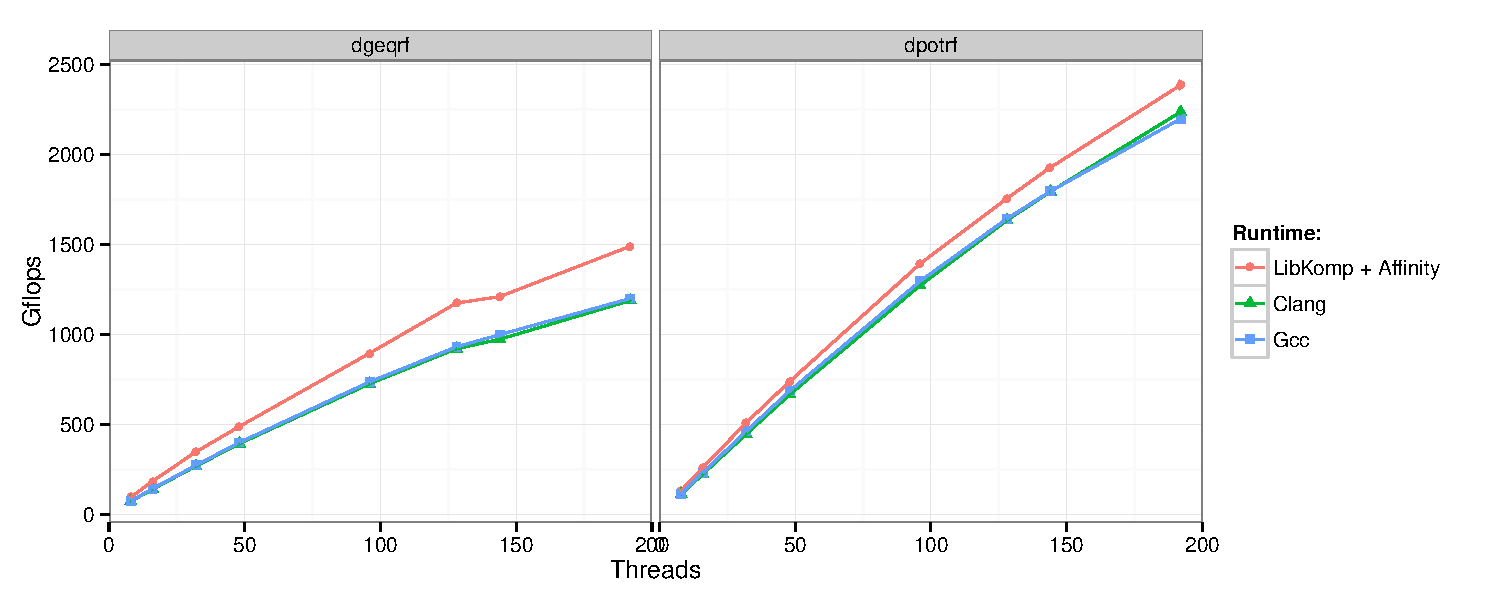
\includegraphics[scale=0.6]{./graphs/graph_dpotrf.pdf}
%\vspace*{-2ex}
  \caption{Cholesky et QR sur Intel192 (Gflops). Taille de matrice 32768, taille de bloc 512}
\label{fig:eval-cholesky}
%\vspace*{-4ex}
\end{figure}

Afin de palier au manque de distribution de données dans les supports exécutifs
de Gcc et de Clang, les données ont été distribuées via \textit{numactl} pour
ces expériences.

L'impact de l'affinité sur les performances est très clair : distribuer les données
par "bloc" et assurer un ordonnancement hiérarchique au plus proche des données écrites offre
de bien meilleures performances que de distribuer les données par "page" (ce que fait
numactl), sans faire attention à la localité des données.


Cette affirmation est à moduler en fonction de la taille de matrice et de bloc :
si la taille de bloc est trop petite, le temps économisé sur le transfert
de données n'est pas significatif et les performances sont équivalentes à celles d'un
support exécutif utilisant une stratégie aléatoire de vol de travail (ce qui est
le cas de ceux de Clang et Gcc).


Sur Intel48 la différence de performance est beaucoup moins flagrante, néanmoins
on peut observer un effet sur l'énergie consommée. La table~\ref{kastors_affinity_pkg}
récapitule les performances, l'énergie consommée par l'ensemble du processeur (PKG),
et celle consommée par la DRAM, en fonction du support exécutif et de la taille de matrice.

\begin{table}[!t]
  \caption{Performances et énergie (Joules) consommée sur 48 threads d'Intel48}
{\small
%\vspace*{-2ex}
\label{kastors_affinity_pkg}
\centering
\begin{tabular}{|c|c|c|c|c|c|c|c|}
\hline
Taille& \multirow{2}{*}{Runtime} & \multicolumn{3}{c|}{dpotrf}  & \multicolumn{3}{c|}{dgeqrf}\\
%\hline
                \cline{3-8}
                (bloc) & & GFlop/s &  E(PKG) & E(DRAM) & GFlop/s & E(PKG) & E(DRAM)\\
\hline
\multirow{3}{*}{16384 (256)}
&Clang           & 665.94 & 796.52  & 80.00 & 455.75 & 4942.94 & 539.80\\
&Gcc             & 682.10 & 787.09  & 83.51 & 470.03 & 4633.48 & 498.07\\
&Komp + Affinity & 677.91 & 784.54  & 73.80 & 471.10 & 4573.89 & 481.64\\
\hline
\multirow{3}{*}{32768 (512)}
&Clang           & 737.93 & 6284.87 & 682.36 & 503.02 & 36901.91 & 4321.06\\
&Gcc             & 746.41 & 6005.53 & 635.87 & 502.82 & 35797.91 & 4166.94\\
&Komp + Affinity & 750.09 & 5866.55 & 599.66 & 508.12 & 34964.64 & 4058.75\\
\hline
\end{tabular}
%\vspace*{-4ex}
}
\end{table}

On peut observer que le support exécutif avec affinité n'est pas significativement meilleur
que ceux de Gcc et Clang, par contre l'énergie consommée par le package du processeur
est plus faible.

Évidemment quand les performances sont légèrement meilleures on peut s'attendre
à ce que l'énergie consommée soit plus faible vu que le temps d'exécution est
plus court.
Or même dans certains cas où les performances de la version avec affinité sont
en retrait, la consommation énergétique est plus faible (ce qui est d'autant plus
vrai quand les performances sont équivalentes).
Une partie de cela est probablement du au fait que l'affinité permet dans tous les
cas de diminuer la consommation énergétique de la DRAM.

Ce comportement est mis en valeur dans la figure~\ref{fig:eval-dram-cholesky},
illustrant la puissance consommée par la DRAM au cours d'une exécution
de Cholesky sur une matrice de taille 32768 (taille de bloc 512).


\begin{figure}[t]
%\vspace*{-4ex}
  \centering
  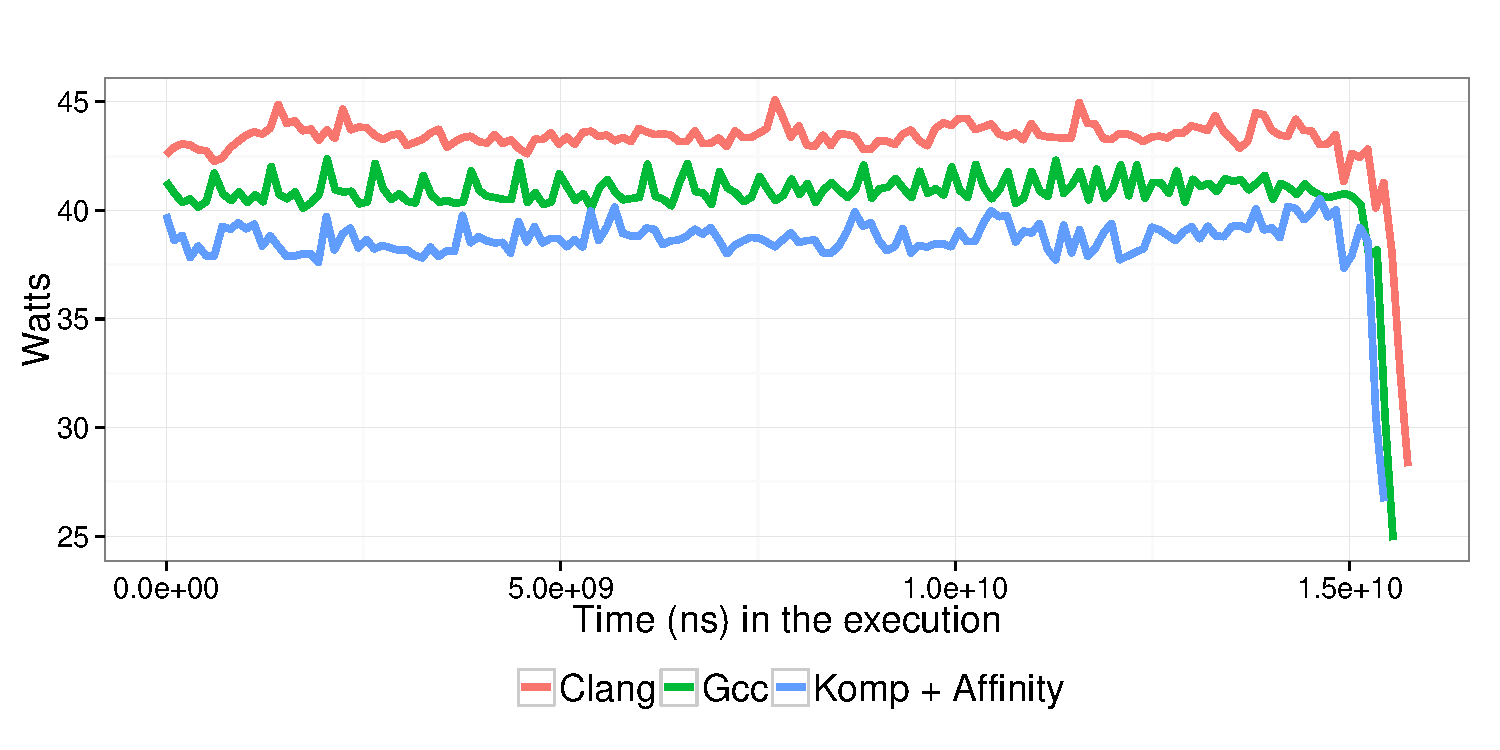
\includegraphics[scale=0.5]{./graphs/graph_energy_dram_dpotrf.pdf}
%\vspace*{-2ex}
  \caption{Consommation (Watts) de la DRAM au cours d'un Cholesky sur Intel48}
\label{fig:eval-dram-cholesky}
%\vspace*{-5ex}
\end{figure}



\section{État de l'art}
%\vspace*{-2ex}
\label{sec:related-work}

De nombreux projets de recherche se sont intéressés à l'exécution d'applications
OpenMP sur des machines NUMA.  

À l'Université de Houston des chercheurs ont travaillés sur l'amélioration de l'affinité mémoire des
régions parallèle et boucles sur des architectures
hiérarchiques~\cite{Marowka:2004:OAD:1064428.1064431}; ainsi que sur l'alignement
des tâches et des données sur des partitions logiques de
l'architecture appelées \textit{locations}~\cite{Huang-Chapman-locality-OpenMP}.

Drebes et al.~\cite{Drebes:2014:TDS:2658949.2641764} ont proposés des techniques
d'ordonnancement pour contrôler le placement des tâches et des données, pour
tirer parti de la localité des données. Ils ont implémenté ces techniques
dans OpenStream, un modèle de programmation par flot de données.
Leur approche se place du point de vue de l'ordonnanceur et ne permet pas à
l'utilisateur d'avoir de la flexibilité dans le placement des données.
Olivier et al.~\cite{Olivier:2012:CMW:2388996.2389085}
ont introduit des queues de tâches OpenMP au niveau des noeuds, appelés
\textit{locality domains}, pour améliorer la localité des tâches vis à vis de
leur données sur des architectures NUMA.
Le placement et la localité des données sont obtenus implicitement en considérant la politique
d'allocation \emph{first-touch} du système.

%Le support exécutif ne maintient pas
%d'information concernant l'affinité des tâches et des données pendant l'exécution,
%et le placement des données est obtenu implicitement en considérant la politique
%d'allocation \emph{first-touch} du système, et la localité des données est assurée en
%ordonnançant les tâches sur les même \textit{locality domains}.

Enfin l'équipe Runtime de l'Université de Bordeaux a proposée le support
exécutif ForestGOMP~\cite{BroFurGogWacNam10IJPP}, qui utilise une API pour
exprimer des affinités entre les régions parallèle OpenMP et des données allouées
dynamiquement. Les affinités mémoire sont déterminées dynamiquement et peuvent
être prise en compte dans l'équilibrage de charge.


%\vspace*{-2ex}
\section{Conclusion et travaux à venir}
%\vspace*{-2ex}
\label{sec:related_work}

Les environnements de programmation à base de tâches tels qu'OpenMP sont devenus
un moyen standard de programmer des systèmes NUMA à large échelle.
Ils offrent au programmeur un moyen d'exprimer du parallélisme à grain fin,
qui peut être associé dynamiquement à la topologie de l'architecture.
OpenMP a récemment évolué pour permettre d'exprimer les dépendances de données
entre tâches.

Cet article présente une nouvelle clause |affinity| offrant plus de flexibilité
au programmeur pour exprimer le lien qui existe entre une tâche et ses données.
Les résultats expérimentaux montrent d'une part qu'une telle clause permet
d'offrir des performances qui n'étaient avant atteignables qu'avec des programmes
itératif (Stencil) ; et d'autre part que les performances des
applications d'algèbre linéaire peuvent directement en bénéficier lorsque
l'architecture cible est fortement impactée par les problématiques NUMA.
À court terme des collaborations avec d'autres personnes et équipes sont prévues
pour offrir des observations plus exhaustives du point de vue de l'énergie.

%\vspace*{-2ex}
\section*{Remerciements}
%\vspace*{-2ex}
Ce travail est réalisé dans le cadre du projet ELCI, un projet collaboratif Français financé par le FSN ("Fond pour la Société Numériqe"), qui associe des partenaires académiques et industriels pour concevoir et produire un
environnement logiciel pour le calcul intensif.

\bibliography{Bib/paper.bib}

\end{document}



